\documentclass[pdf]{beamer}
\mode<presentation>{} 
%% preamble
\usepackage{slidepacks}
\usepackage{hyperref}
\setbeamertemplate{caption}[numbered]
\usepackage[justification=centering]{caption}

\newcommand{\Lap}{\mathcal{L}}

\usetheme{Ilmenau}

\definecolor{camred}{RGB}{140, 21, 21} % camred (primary)
\definecolor{camlg}{RGB}{236, 236, 236}
\definecolor{camdg}{RGB}{217, 217, 217}
\setbeamercolor{palette primary}{bg=camred,fg=white}
\setbeamercolor{palette secondary}{bg=camdg,fg=black}
\setbeamercolor{palette tertiary}{bg=camlg,fg=black}
\setbeamercolor{palette quaternary}{bg=camlg,fg=black}
\setbeamercolor{structure}{fg=camred} % itemize, enumerate, etc
\setbeamercolor{section in toc}{fg=camred} % TOC sections

\definecolor{evandp}{RGB}{120, 66, 119}
\definecolor{evanlp}{RGB}{251, 241, 251}

\setbeamercolor{block title}{use=structure,fg=white,bg=evandp}
\setbeamercolor{block body}{use=structure,fg=black,bg=evanlp}

\beamertemplatenavigationsymbolsempty

\title[Randoms Correction]{Randoms Correction Techniques \\ on the Gen II System}
\author[Eegan Ram]{Eegan Ram, Dr. Garry Chinn \texorpdfstring{\\}{}
\texorpdfstring{Stanford University}{}}
\date{\today}

\begin{document}


\begin{frame}
\thispagestyle{empty}          % prevents page numbering on the title slide
\titlepage
\end{frame}
\addtocounter{framenumber}{-1} % don't count title slide in the page numbering

\section{Introduction}

\begin{frame}{Randoms Correction}
    \begin{itemize}
        \item How many of the coincidences measured on a certain LOR are `random coincidences?'
        \item We use this information to advise image reconstruction.
    \end{itemize}
\end{frame}

\begin{frame}{Methods}
    \begin{itemize}
        \item Delayed-Window (DW)
        \item Singles-Rate (SR)
        \item Singles-Prompts (SP) - 2016, new to our group
        \item Singles-Prompts with Multiple Coincidence Correction - new
    \end{itemize}
\end{frame}

\begin{frame}{Delayed-Window (DW)}
    \begin{figure}[H]
        \centering
        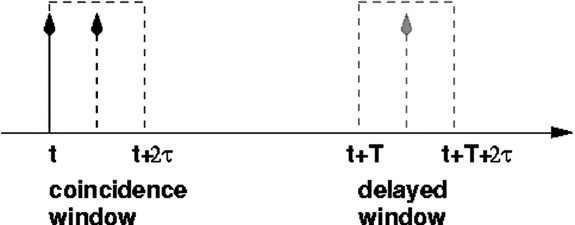
\includegraphics[width=0.8\textwidth]{figures/dwdemo.png}
    \end{figure}
    \begin{itemize}
        \item Every time you open a prompt window, also open a delayed window.
        \item A count in the DW $=$ random coincidence on that LOR.
        \item Currently implemented on hardware.
    \end{itemize}
\end{frame}

\begin{frame}{Singles-Rate (SR)}
    $$R_{ij} = 2 \rn{tau}{\tau} \rn{si}{S_i} \rn{sj}{S_j}$$
    \customanno{tau.north}{3em}{50}{coincidence window}{rotate=5}
    \customanno{si.south west}{3em}{-160}{\# singles in crystal $i$}{xshift=-7em, yshift=-0.7em}
    \customanno{sj.south east}{3em}{-40}{\# singles in crystal $j$}{}

    \vspace{2em}

    \begin{itemize}
        \item Estimates random coincidences from \# singles counts. 
        \item Requires singles acquisition.
    \end{itemize}
\end{frame}

\begin{frame}{Singles-Prompts (SP)}
    $$R_{ij}^{SP} = \frac{2 \tau e^{-(\lambda + S) \tau}}{(1 - 2 \rn{lam}{\lambda} \tau)^2 } \left(S_i - e^{(\lambda + S) \tau} \rn{prompti}{P_i}\right) \left(S_j - e^{(\lambda + S) \tau} P_j\right)$$
    \customanno{prompti.north}{3em}{30}{\# prompts in crystal $i$}{}
    \customanno{lam.south east}{4em}{-40}{Solution to $2 \tau \lambda^2 - \lambda + S - P e^{(\lambda + S)\tau}$}{}

    \vspace{3em}

    \begin{itemize}
        \item Estimates random coincidences from \# singles counts \textit{and} prompts counts.
        \item Requires singles acquisition.
        \item Incorporates prompt information for improved accuracy (second order).
    \end{itemize}

\end{frame}

\begin{frame}{Singles-Prompts Extension}
    $$R_{ij} = R_{ij}^{SP} \cdot \frac{\rn{prodk}{\prod_k} e^{-S_k \tau^2 / T}}{e^{-S_i \tau^2 / T} e^{- S_j \tau^2 / T}}$$
    \customanno{prodk.north}{3em}{30}{\# sum over all crystals $k$}{}

    \vspace{2em}

    \begin{itemize}
        \item Note: typically a ``downwards'' correction.
    \end{itemize}
\end{frame}

\section{Basic Comparison}

\begin{frame}{Cylindrical Simulated Source - Sum over Crystals}
    \begin{figure}
        \centering
        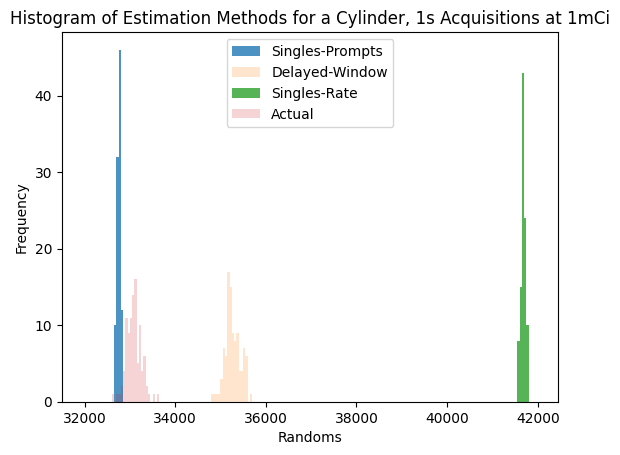
\includegraphics[width=0.8\textwidth]{figures/hist1mCi.png}
    \end{figure}
\end{frame}

\begin{frame}{Cylindrical Source - SP Extension}
    \begin{itemize}
        \item SP nearly always underestimates $R_{ij}$, downcorrection unhelpful.
        \item Downcorrection was extremely small $\approx 10^{-4}$.
        \item Not worth using?
    \end{itemize}
\end{frame}

\section{Subtraction}

\begin{frame}{Flangeless Esser PET Phantom}
    \begin{figure}
        \centering
        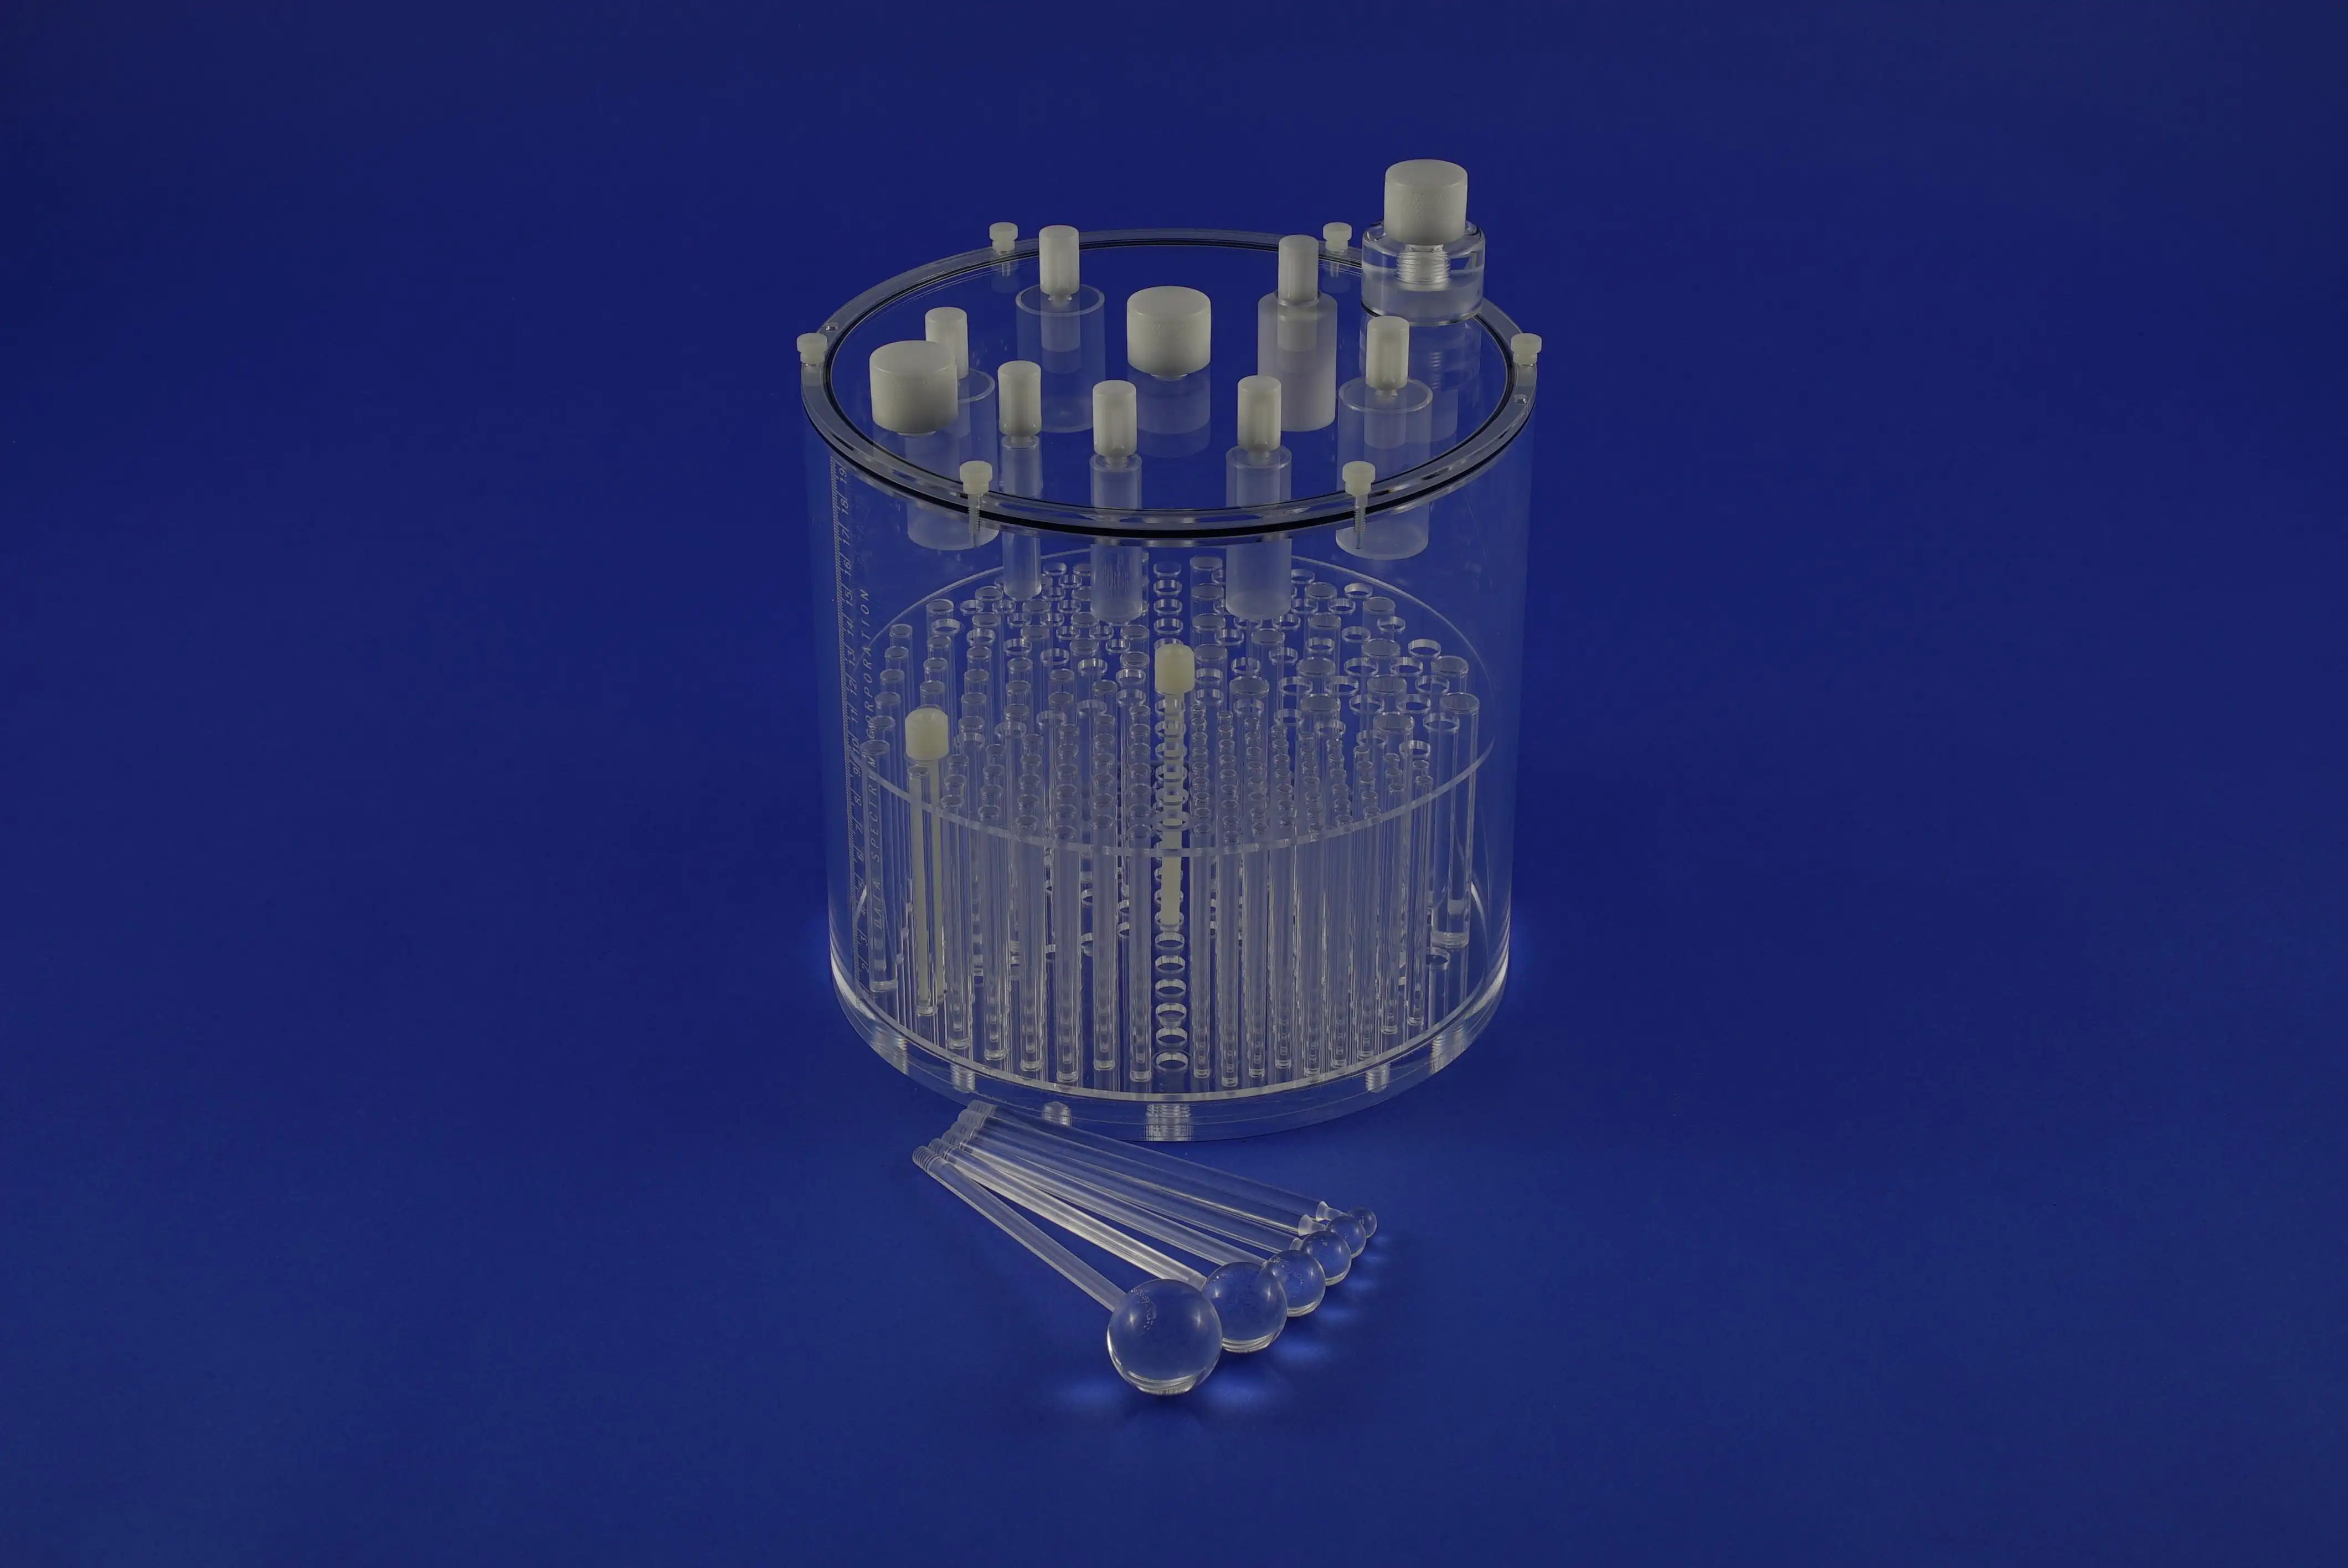
\includegraphics[width=0.6\textwidth]{figures/flangeless.png}
    \end{figure}

    \begin{itemize}
        \item $48 \mu Ci$ over fillable capsules
        \item $1.5 mCi$ in large volume
    \end{itemize}
\end{frame}

\begin{frame}{Methods for Removing Randoms}
    \begin{enumerate}
        \item Subtraction Method: Remove coincidences on same LOR closest to TOF
        \item Contamination List: $\frac{\text{num of randoms on LOR}}{\text{num of prompts on LOR}}$
    \end{enumerate}
    
    \vspace{0.25in}

    (1) is compatable with CUDA Recon (current model), (2) requires parallelproj.

    \vspace{0.25in}

    Note: for subtraction with SP, we assume a uniform distribution across TOF.
\end{frame}

\begin{frame}{Annulus: `True' Subtraction (Sampled LOR 0-10)}
    \begin{figure}
        \centering
        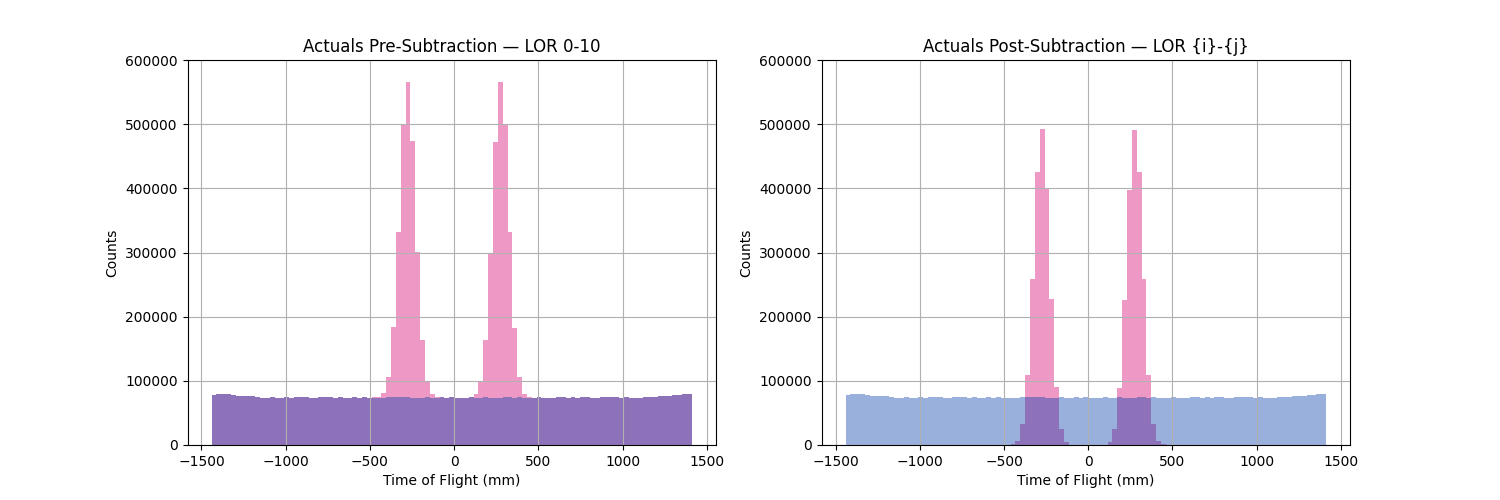
\includegraphics[width=\textwidth]{figures/0_10_actual.png}
    \end{figure}

    \begin{itemize}
        \item Pink: coincidences
        \item Blue: estimated random coincidences
    \end{itemize}
\end{frame}

\begin{frame}{Annulus: DW Subtraction}
    \begin{figure}
        \centering
        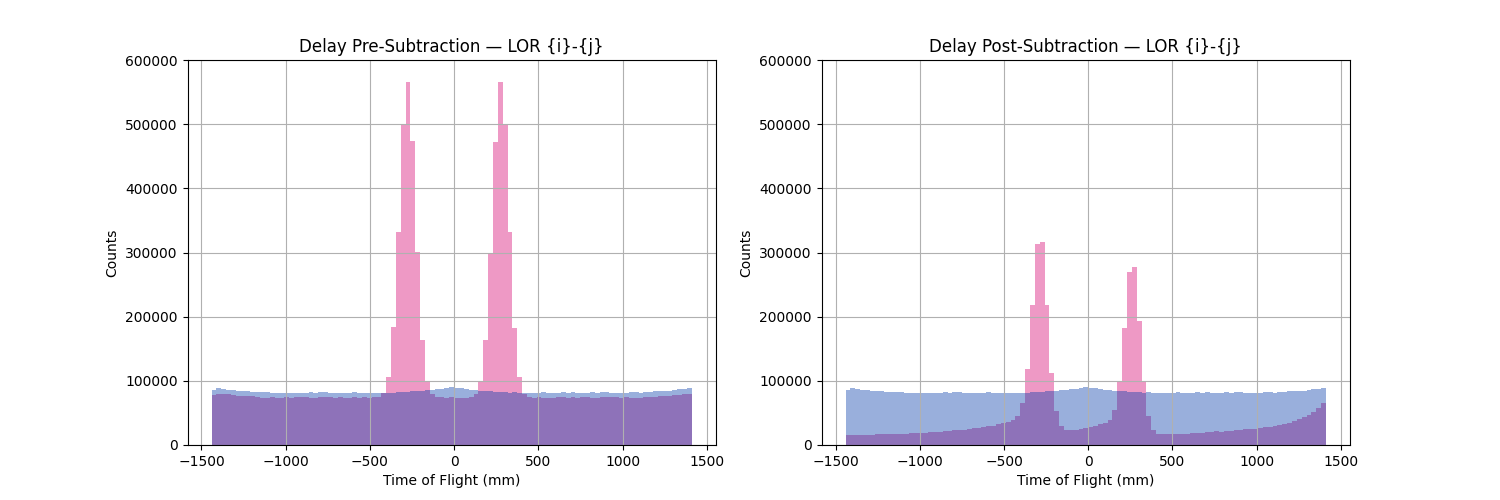
\includegraphics[width=\textwidth]{figures/0_10_delay.png}
    \end{figure}
    \begin{itemize}
        \item Pink: coincidences
        \item Blue: estimated random coincidences
    \end{itemize}
\end{frame}

\begin{frame}{Annulus: SP Subtraction}
    \begin{figure}
        \centering
        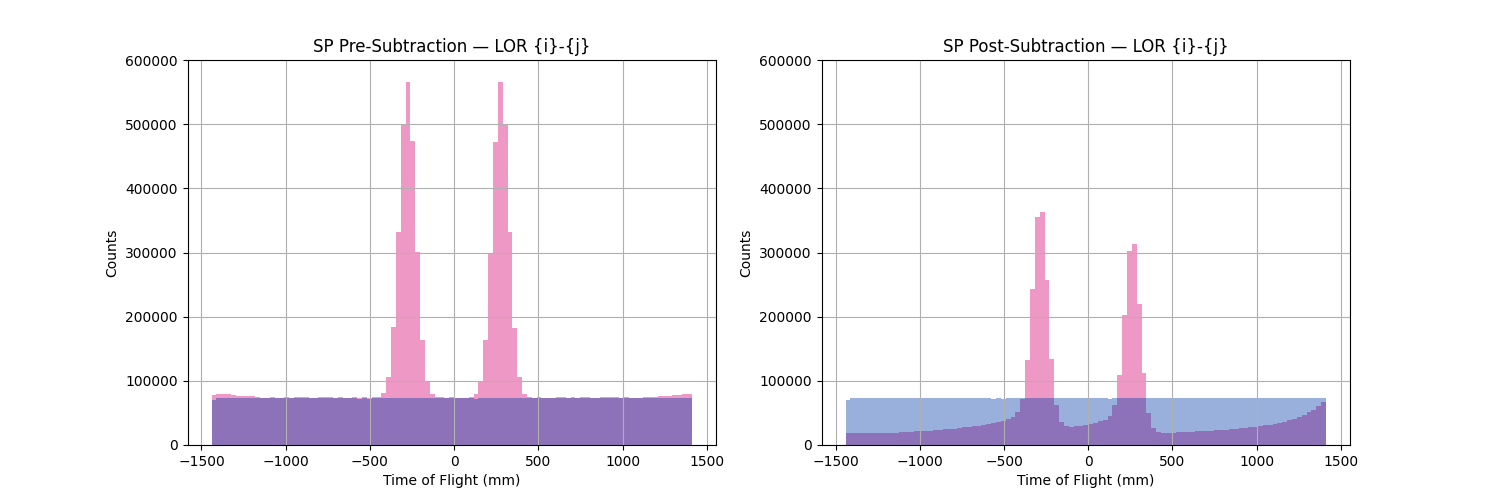
\includegraphics[width=\textwidth]{figures/0_10_sp.png}
    \end{figure}
    \begin{itemize}
        \item Pink: coincidences
        \item Blue: estimated random coincidences
    \end{itemize}
\end{frame}

\begin{frame}{Annulus: Trues Kept}
    \begin{figure}
        \centering
        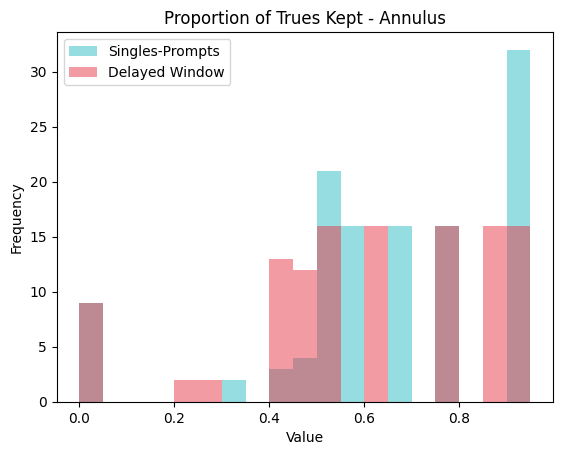
\includegraphics[width=0.65\textwidth]{figures/trueskeptann.png}
    \end{figure}
    Mean: 0.645 (SP), 0.602 (DW)
\end{frame}

\begin{frame}{Annulus: Randoms Caught}
    \begin{figure}
        \centering
        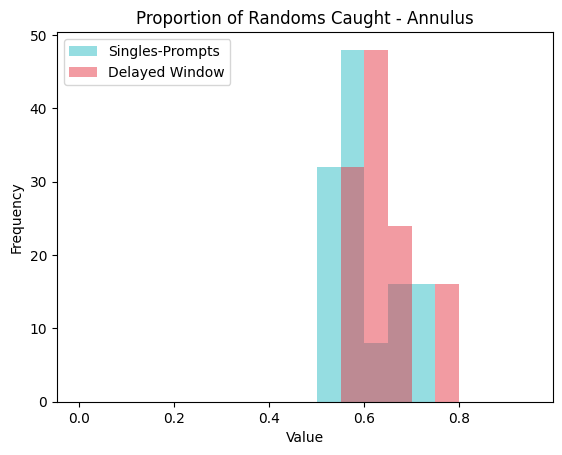
\includegraphics[width=0.65\textwidth]{figures/randomscaughtann.png}
    \end{figure}
    Mean: 0.604 (SP), 0.641 (DW)
\end{frame}

\begin{frame}{Subtraction - Esser Phantom}

    Mean values:
    \begin{table}[]
        \begin{tabular}{lllll}
        \multicolumn{1}{l|}{}               & SP     & DW     &  &  \\ \cline{1-3}
        \multicolumn{1}{l|}{Trues Kept}     & 88.1\% & 86.5\% &  &  \\
        \multicolumn{1}{l|}{Randoms Caught} & 52.0\% & 50.8\% &  &  \\
                                            &        &        &  & 
        \end{tabular}
    \end{table}

    Marginal improvement.
\end{frame}


\section{Contamination}

\begin{frame}{Contamination Analysis - Esser Phantom}
    \begin{figure}
        \centering
        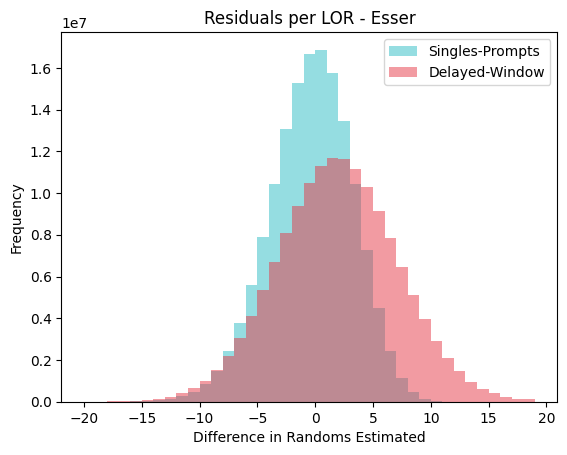
\includegraphics[width=0.8\textwidth]{figures/esserdiff.png}
    \end{figure}
\end{frame}

\begin{frame}{Contamination Analysis - Esser Phantom}
    \begin{table}
        \begin{tabular}{lllll}
        \multicolumn{1}{l|}{}               & SP     & DW     &  &  \\ \cline{1-3}
        \multicolumn{1}{l|}{Mean}     & -0.33 & 1.43 &  &  \\
        \multicolumn{1}{l|}{STDev} & 3.57 & 5.18 &  &  \\
                                            &        &        &  & 
        \end{tabular}
    \end{table}
\end{frame}

\section{Conclusion}

\begin{frame}{Key Findings}
    \begin{itemize}
        \item SP and DW methods have similar performances when using our current subtraction method (SP marginally better).
        \item With the use of the contamination list method, SP has a slight advantage.
    \end{itemize}
\end{frame}

\begin{frame}{Next Steps}
    \begin{itemize}
        \item Reconstruct the relevant images with both methods, need to ensure parallelproj works properly.
        \item Calculate SNR, other stats from those images to see if the difference using contamination list is worth collecting singles.
    \end{itemize}
\end{frame}


\section{Acknowledgements}

\begin{frame}{Acknowledgements}
\begin{itemize}
\item Dr. Garry Chinn
\item Dr. Nasir Ullah
\item Sarah Zou
\item Professor Craig Levin
\item James Ho
\item Grant Hee-Sung Park
\end{itemize}
\end{frame}

\end{document}